\section{Clustering}

\begin{breakbox}
\boxtitle{k-means:}

\begin{enumerate}
	\item Arbitrarily choose k instances
	\item Define these instances as initial cluster centers
	\item Determine each instance's distance to the cluster centers
	\item Assign each instance to it's nearest cluster center
	\item If no change in cluster allocation: \textbf{Exit}
	\item Calculate the mean for each cluster:
	$\frac{\text{sum of all x-coords of instances}}{\text{number of instances}} = \text{new x-coordinate}$
	$\frac{\text{sum of all y-coords of instances}}{\text{number of instances}} = \text{new y-coordinate}$
\end{enumerate}

\textbf{Advantages/Disadvantages:}
\begin{itemize}
	\item Fast, converges easily (stops at local optimums)
	\item result depends heavily on initialization
	\item clusters are heavily impacted by outliers
\end{itemize}

k-medoid uses always a cluster medoid (center is a always an instance, not a non-existing mean point). The ''most central'' instance becomes the new cluster center. More robust regarding outliers. Center is chosen as the instance with the lowest costs (error) if this instance is chosen.

E = total error of allocation, $C_j$ is cluster j with center $c_j$ and $p$ any non-center instance.
\begin{center}
	$E=\sum_{j=1}^{k} \sum_{p \in C_j}^{} |p-c_j|$
\end{center}

\end{breakbox}

\begin{breakbox}
\boxtitle{Distance of Binary Data:}
Distance cannot be calculated on ordinal or nominal scales.

\begin{center}
	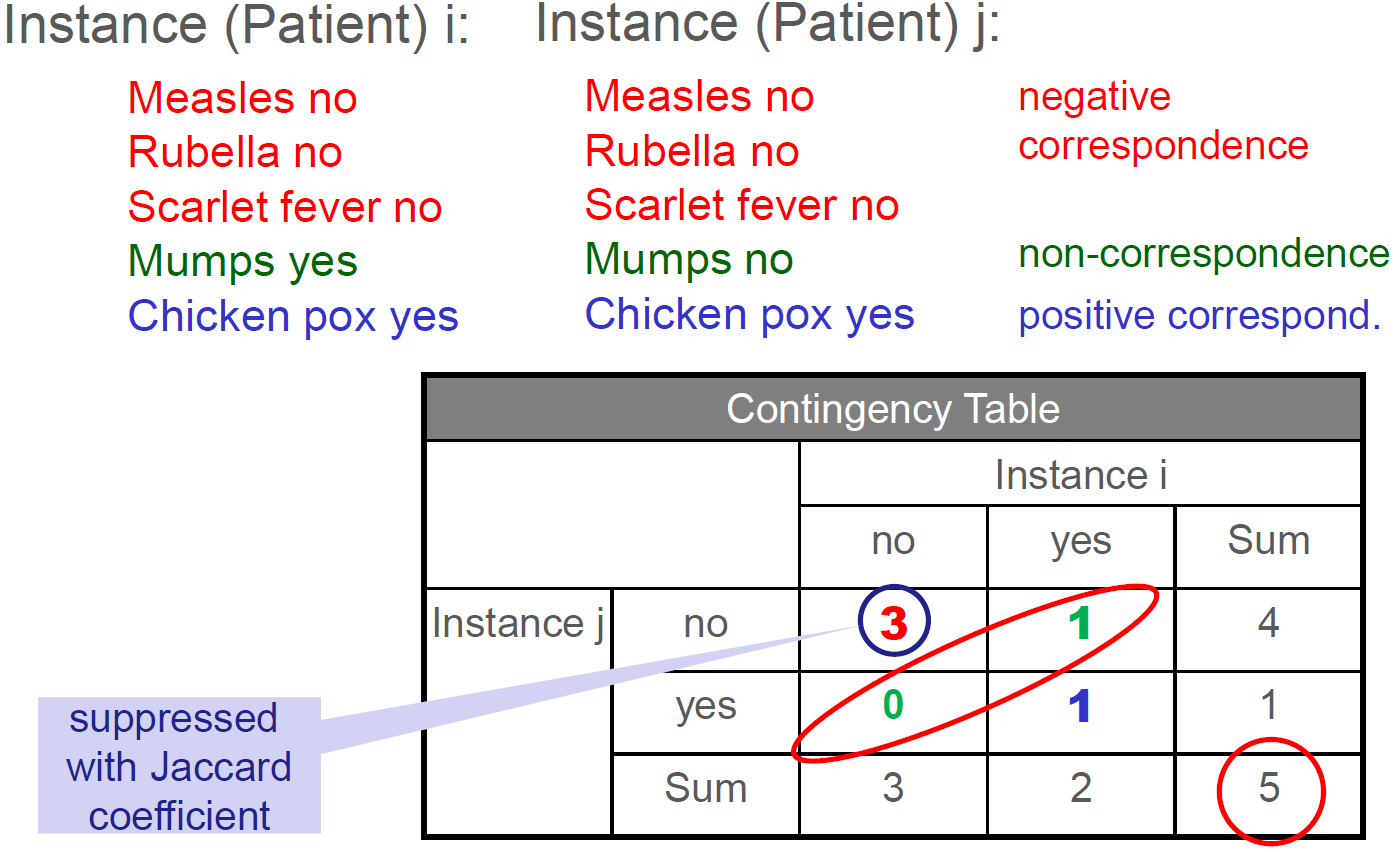
\includegraphics[width=.15\textwidth]{slides_images/clustering_binary_distance.png}
\end{center}

Jaccard coefficient is like a distance: $d=\frac{0+1}{5-3} = \frac{1}{2}$

\end{breakbox}



\begin{breakbox}
\boxtitle{Distance of Nominal Data}

\begin{itemize}
	\item Nominal scale:
		\begin{itemize}
			\item red, yellow, blue, green, white
			\item food, health-care, toys, electronics
			\item $d=\frac{\# \text{attr} - \# \text{correspondences}}{\# \text{attr}}$			
		\end{itemize}
	\item Ordinal scale
		\begin{itemize}
			\item rank nominal data by some order, e.g. gold, silver, bronze
			\item calculate as usual, e.g. by Euclidean or Manhattan distance
		\end{itemize}
\end{itemize}
\end{breakbox}



\begin{breakbox}
\boxtitle{Approaches for Outlier Detection:}

\begin{itemize}
	\item Statistical Distribution-Based Outlier Detection
		\begin{itemize}
			\item assuming that attribute values answer to statistical measures, e.g. an overlap of Gaussian distributions
			\item if probability of distribution membership is very low $\implies$ outlier		
		\end{itemize}
	\item Density-Based Outlier Detection
		\begin{itemize}
			\item most attribute values of all other instances are beyond a pre-defined minimum distance $\implies$ outlier
		\end{itemize}
	\item Deviation-Based Outlier Detection
		\begin{itemize}
			\item Definition of a total dissimilarity measure for all instances		
			\item if an instance's exclusion reduces dissimilarity significantly $\implies$ outlier
		\end{itemize}
\end{itemize}
\end{breakbox}



\begin{breakbox}
\boxtitle{EM Algorithm:}

\textbf{E}xpectation-\textbf{maximization} algorithm for membership by probability. \textbf{Determines the number of clusters automatically!}

\begin{center}
	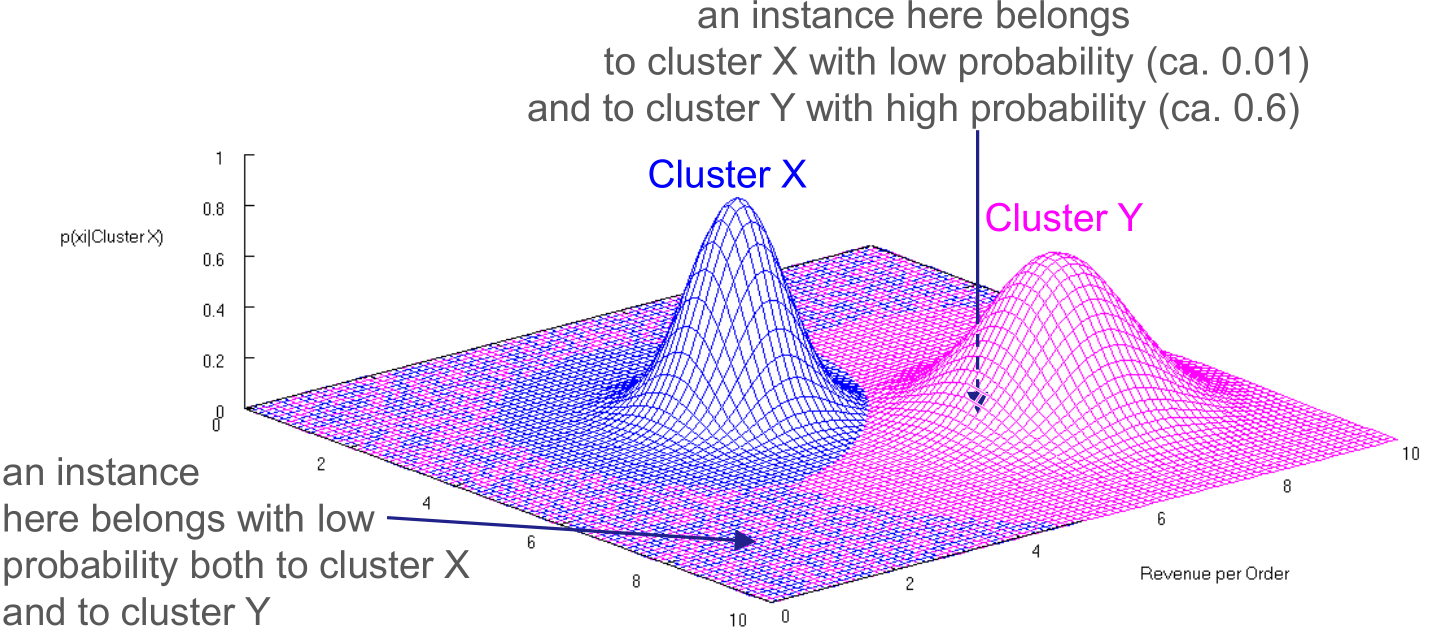
\includegraphics[width=0.15\textwidth]{slides_images/membership_by_probability_em}
\end{center}

\begin{itemize}
	\item Initial guess of k distribution curves (=the model)
		\begin{itemize}
			\item random model parameters $\mu$ and $\sigma$
		\end{itemize}
	\item iteratively take 2 steps
		\begin{enumerate}
			\item Expectation: calculate ''expected'' cluster membership
			\item Maximization: re-estimate model parameters (refine memberships)
		\end{enumerate}
	\item usage of a maximum likelihood (ML) function; describes the probability that instances belong to clusters
	\item algorithm ends if function cannot be increased anymore
\end{itemize}

Goal: maximize the probability of a cluster allocation. To that end we maximize the product from the following probabilities:
\begin{itemize}
	\item $p(A)$: Cluster A's proportion of the total set of instances or probability for any instance to be in Cluster A.
	\item $p(x_i|A)$: probability for $x_i$ to be in Cluster A.
\end{itemize}

Bayes' theorem: $p(A|x_i) = \frac{p(x_i|A) \cdot p(A)}{p(x_i)}$

Do this for all clusters (an instance belongs to all clusters): $p(A) \cdot p(x_i|A) + p(B) \cdot p(x_i|B) + \cdots$

For all instances (to asses overall model fitness), this is the maximum likelihood function and needs to be maximized:
\begin{center}
	$\prod_{i}{}(p(A) p(x_i|A) + p(B) p(x_i|B) + \cdots)$
\end{center}

\begin{itemize}
	\item $p(A) \cdot p(x_i|A)$ is the expectation that $x_i$ is in cluster A
	\item Summing up expectations for one instance $x_i$ over all clusters delivers the overall expectation that $x_i$ is in clusters at all (=1 is the ideal case)
	\item The product from the ML function is the combined expectation of all instances $x_1, x_2, \cdots x_i$ belonging to clusters somewhere
	\item Thus the ML function expresses the overall probability that instances are covered by clusters: Where are the clusters most likely to be?
	\item Constantly improved with each iteration
\end{itemize}

\textbf{Advantages:}
\begin{itemize}
	\item Evaluation of number of clusters k
	\item Robust regarding outliers. An outlier would be allocated to every cluster but with very little probability. So the outlier has very little influence on model parameter adjsutment.
\end{itemize}
\end{breakbox}




\begin{breakbox}
\boxtitle{COBWEB Hierarchical Clustering:}
\end{breakbox}



\begin{breakbox}
\boxtitle{DENCLUE:}
\textbf{DEN}sity-based \textbf{CLU}st\textbf{E}ring: Each function has a influence function. Influence is high at the instance's location and diminishes with growing distance.

Two parameters:
\begin{itemize}
	\item $\sigma$
		\begin{itemize}
			\item control the range of an influence function
			\item the higher $\sigma$ the more overlap of influence functions
		\end{itemize}
	\item $\xi$
		\begin{itemize}
			\item threshold for influence considerations
			\item  kind of a ''water level'': only areas with
sufficient influence rise above the level and show as clusters
			\item the higher $\xi$ the smaller get cluster areas
		\end{itemize}
\end{itemize}

\begin{center}
	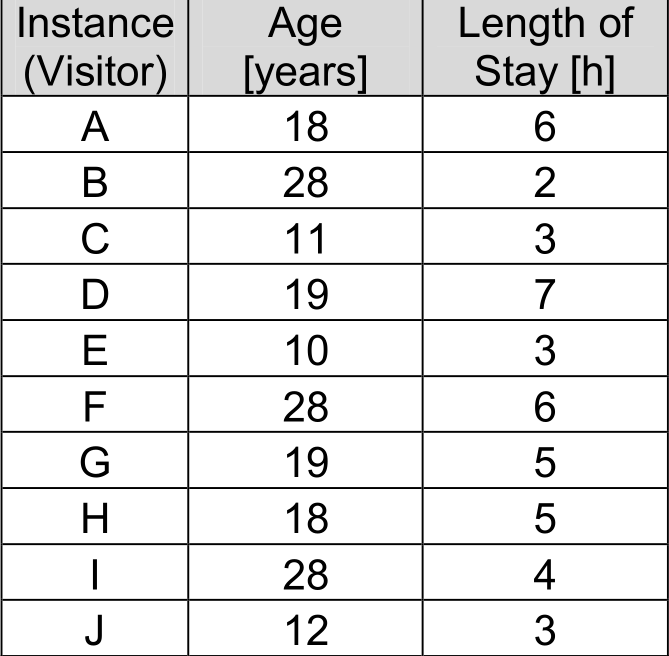
\includegraphics[width=.07\textwidth]{slides_images/denclue_data_table}
\end{center}

Influence function is square wave is given as:

\begin{center}
	$f_{\text{Square}} (x,y) = \begin{cases} 
    	  0 \text{ if} d(x,y) > \sigma \\
	      1 \text{ if} d(x,y) \leq \sigma
	   \end{cases}$
\end{center}

Determine $\sigma$ as well as $\xi$ in order to get exactly two clusters (each covering some instances).

\begin{itemize}
	\item Two clusters means that a cluster should show where the instances E / C / J are located, but no cluster with F / I / B. This implies that some areas at E / C / J are "higher" than the most elevated spot at F / I / B. This can only be the case for 1 $\leq \sigma \le 2$
	\item $\xi$ then has to be greater than 2 and less than 3 in order to let F / I / B be ''swallowed by the
tide'' while E / C / J still rises ''above the flood''.
\end{itemize}

\begin{center}
	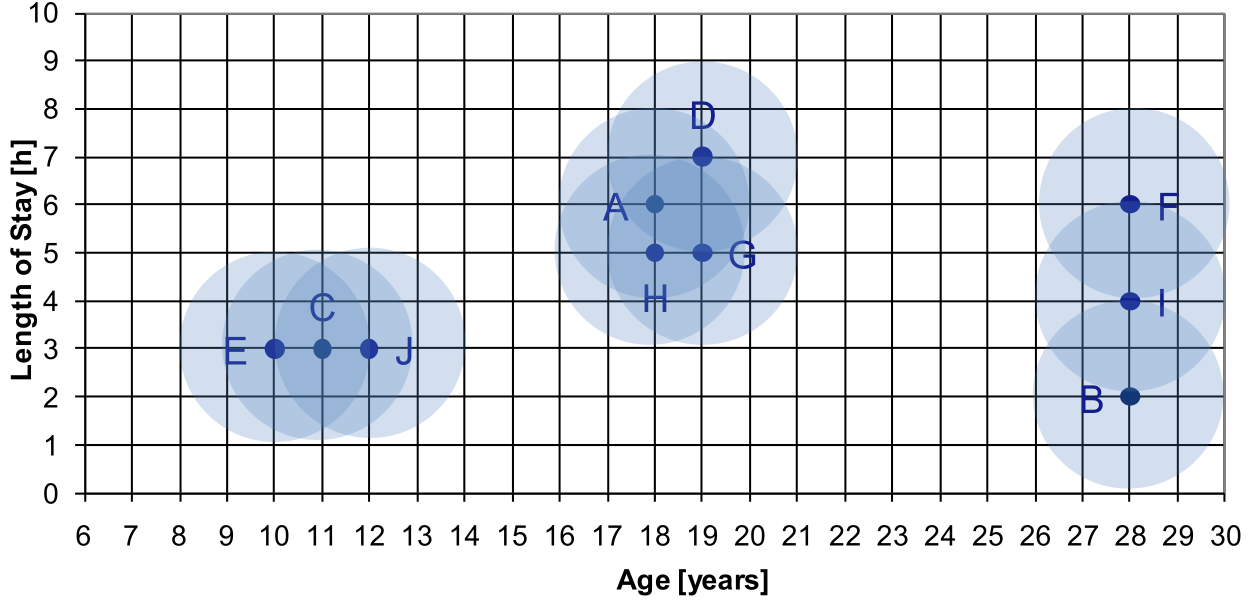
\includegraphics[width=.15\textwidth]{slides_images/denclue_cluster}
\end{center}

\textbf{Instances that are part of a cluster:}
With $2 \le \xi \le 3$, cluster areas need the influence functions of at least 3 instances at the same time to surmount $\xi$. Since $\sigma$ is less than 2 all instances in such cluster areas have to have 2 other instances nearer than distance 2 (only two other instances because each instance's own influence counts as well). This is only the case for instances \textbf{A, C, G, H}. D has only influence from A, but not from G ($\sigma$ is less than 2!). The same applies to E and J.
\end{breakbox}